\subsection{Map}\label{ssec:map}
The map data type stores 2D spatial data, such as images of the Sun and 
inner heliosphere. It provides: a wrapper around a \texttt{numpy} data array, 
the images associated spatial coordinates, and other metadata. The \texttt{Map} 
class provides methods for typical operations on 2D data, such as rotation and 
re-sampling, as well as visualisation.
The \texttt{Map} class also provides a convenient interface for loading data 
from a variety of sources, including from FITS (Flexible Image Transport System) 
files, the standard format for storing image data in solar physics and astrophysics community. 
An example of creating a \texttt{Map} object from a FITS file is shown in 
Listing~\ref{code:aia_1}.

The architecture of the map subpackage consists of a template map called
\texttt{GenericMap}, which is a subclass of \texttt{astropy.nddata.NDData}. 
\texttt{NDData} is a generic wrapper around a \texttt{numpy.ndarray} with a 
\texttt{meta} attribute to store metadata.
As \texttt{NDData} is currently still in development, \texttt{GenericMap} does 
not yet make full use of its capabilities, but this inheritance structure 
provides for future integration with \texttt{astropy}. In order to provide 
instrument- or detector-specific integration, \texttt{GenericMap} is designed
to be subclassed. Each subclass of \texttt{GenericMap} can register 
with the \texttt{Map} creation function, which will then automatically return an instance
of the specific \texttt{GenericMap} subclass dependent upon the data provided. 
SunPy v0.5 has \texttt{GenericMap} specialisations for the following 
instruments: 

\begin{itemize}
\item \textit{Yohkoh}/SXT - SXT: Solar X-ray Telescope \citep{1991SoPh..136....1O, 1991SoPh..136...37T},
\item \textit{SOHO}/EIT and LASCO - SOHO: Solar and Heliospheric Observatory \citep{domingo1995}, EIT: Extreme Ultraviolet Telescope \citep{1995SoPh..162..291D} and LASCO: Large Angle Spectroscopic COronagraph \citep{1995SoPh..162..357B}
\item \textit{RHESSI} - RHESSI: Reuven Ramaty High Energy Solar Spectroscopic Image \citep{2002SoPh..210....3L},
\item \textit{STEREO}/EUVI and COR1/2 - STEREO: Solar TErrestrial RElations Observatory \citep{2005AdSpR..36.1483K}, EUVI: Extreme Ultraviolet Imager \citep{2004SPIE.5171..111W} and COR1/2: CORonagraph 1/2 \citep{2002AdSpR..29.2017H}
\item \textit{Hinode}/XRT - XRT: X-Ray Telescope \citep{2007SoPh..243....3K, 2007SoPh..243...63G}.
\item \textit{PROBA2}/SWAP - PROBA2: PRojects for On Board Autonomy 2 \citep{2013SoPh..286....5S}, SWAP: Sun Watcher Active Pixel \citep{2013SoPh..286...43S}
\item \textit{SDO}/AIA and HMI - HMI: Helioseismic Magnetic Imager, \citep{2012SoPh..275..207S}
\item \textit{IRIS} - IRIS: Interface Region Imaging Spectrograph \citep{2011SPD....42.1512L} SJI (slit-jaw imager) frames.           
\end{itemize}
             
The \texttt{GenericMap} class stores all of the metadata retrieved from the header of
the image file in the \texttt{meta} attribute and provides convenience 
properties for commonly accessed metadata: e.g., \texttt{instrument}, 
\texttt{wavelength} or \texttt{coordinate\_system}.
These properties are dynamic mappings to the underlying metadata and all methods 
of the \textit{GenericMap} class modify the meta data where needed.
For example, if \verb|aiamap.meta[`instrume']| is modified then \verb|aiamap.instrument| 
will reflect this change.
Currently this is implemented by not preserving the keywords of the input data,
instead modifying meta data to a set of ``standard" keys supported by SunPy.
Listing \ref{code:aia_1} demonstrates the quick-look functionality of 
\texttt{Map}.

\begin{listing}[H]
\pythoncode{pycode_map1.txt}
\begin{center}
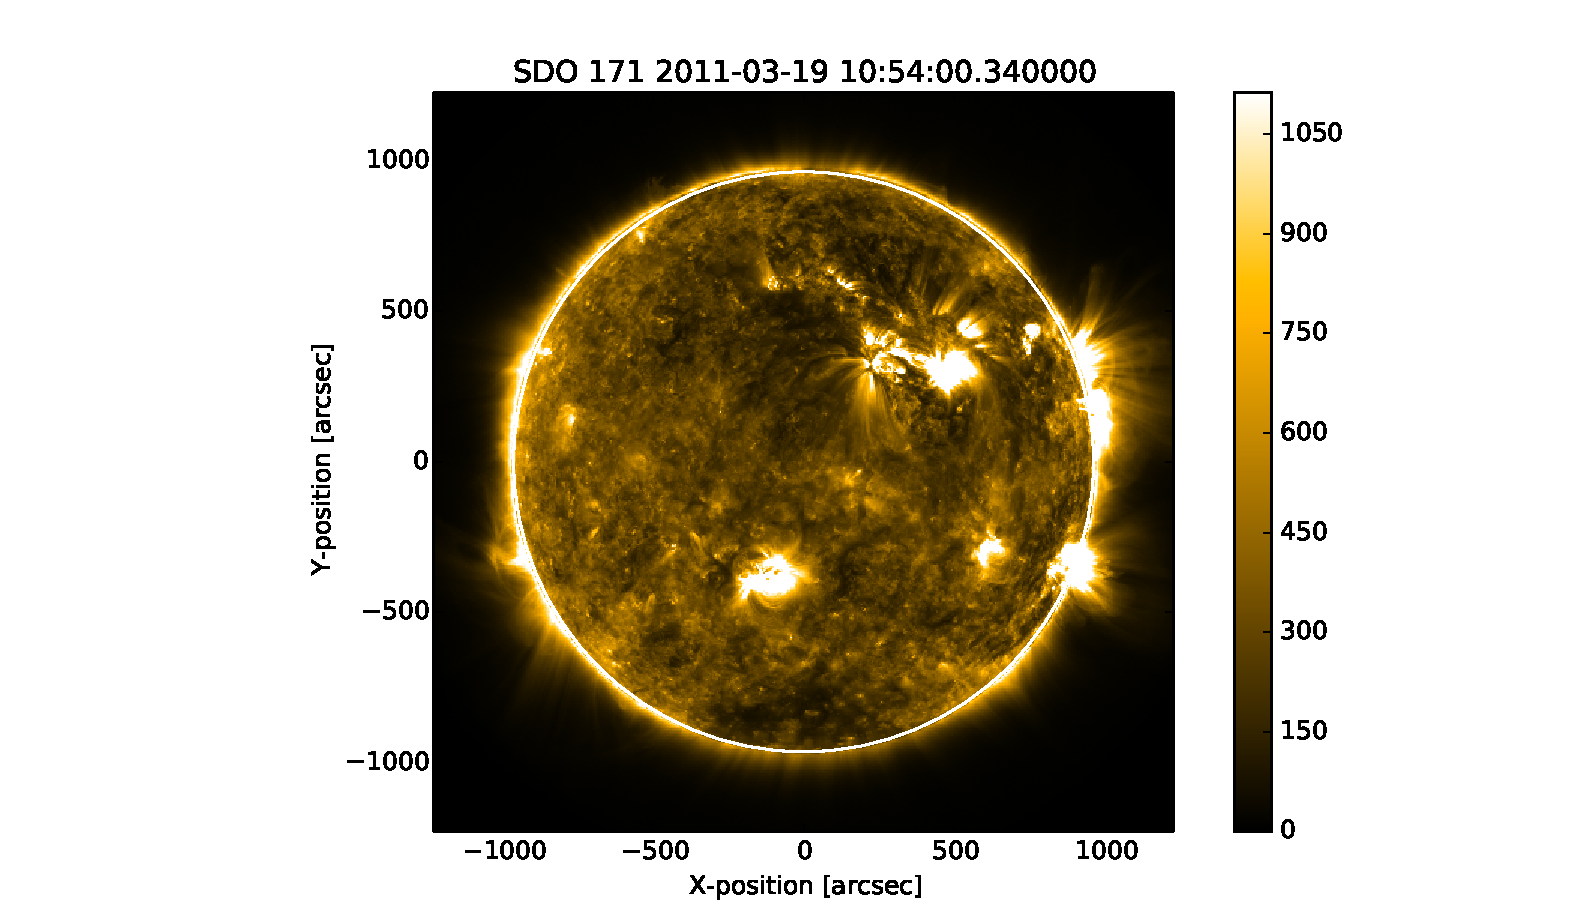
\includegraphics[width=0.8\columnwidth]{aia_map_example}
\end{center}
\caption{Example of the \texttt{AIAMap} specialisation of 
\texttt{GenericMap}. First, a map is created from a sample \textit{SDO}/AIA FITS file. In this case, a demonstration file contained within the SunPy repository is used. A cutout
of the full map is then created by specifying the desired solar-$x$ and solar-$y$ ranges of the plot in data coordinates (in this case, arcseconds), and then a quick-view plot is created with lines of heliographic longitude and latitude over-plotted.}
\label{code:aia_1}
\end{listing}

In addition to the data-type classes, the \texttt{map} subpackage provides two 
collection classes, \texttt{CompositeMap} and \texttt{MapCube}, for 
spatially and temporally aligned data respectively.
\texttt{CompositeMap} provides methods for overlaying spatially aligned 
data, with support for visualisation of images and contour lines overlaid 
upon each other.
\texttt{MapCube} provides methods for animation of its series of \texttt{Map} 
objects. Listings~\ref{code:compmap_1} and \ref{code:mapcube_1} show how to 
interact with these classes.

\begin{listing}[H]
\pythoncode{pycode_map2.txt}
\begin{center}
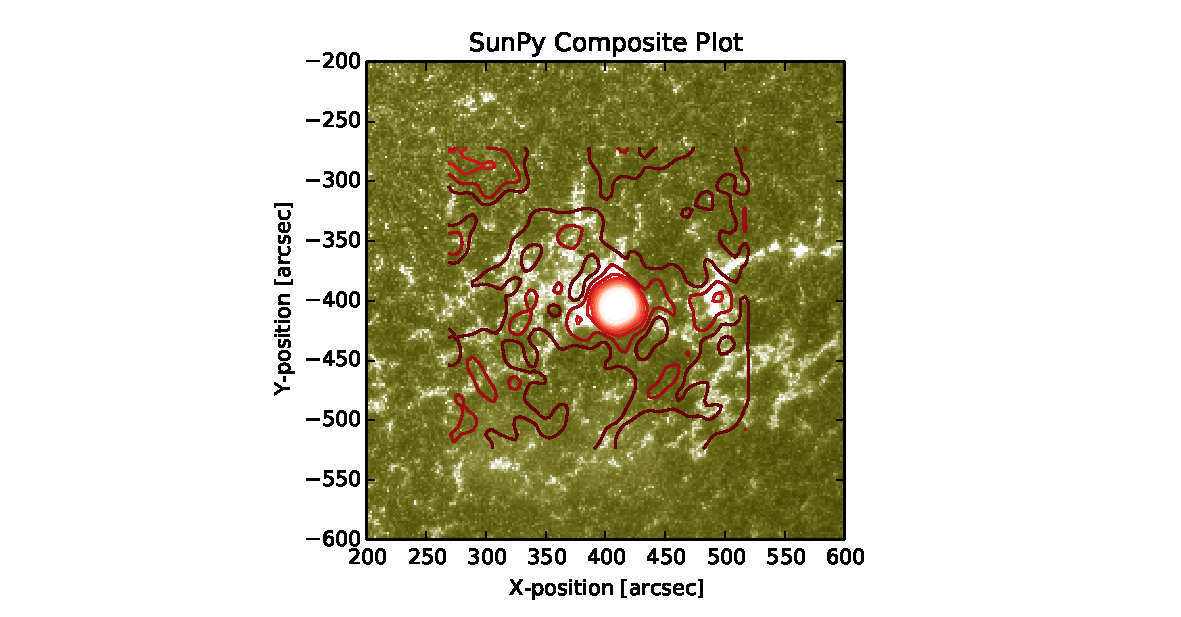
\includegraphics[width=0.8\columnwidth]{comp_map_example}
\end{center}
\caption{Example showing the functionality of \texttt{CompositeMap}, with RHESSI X-ray image data composited
on top of an \textit{SDO}/AIA 1600 $\AA$ image. The \texttt{CompositeMap} is plotted using the integration with the \texttt{matplotlib.pyplot} interface.}
\label{code:compmap_1}
\end{listing}

\begin{listing}[H]
\pythoncode{pycode_map3.txt}
\begin{center}
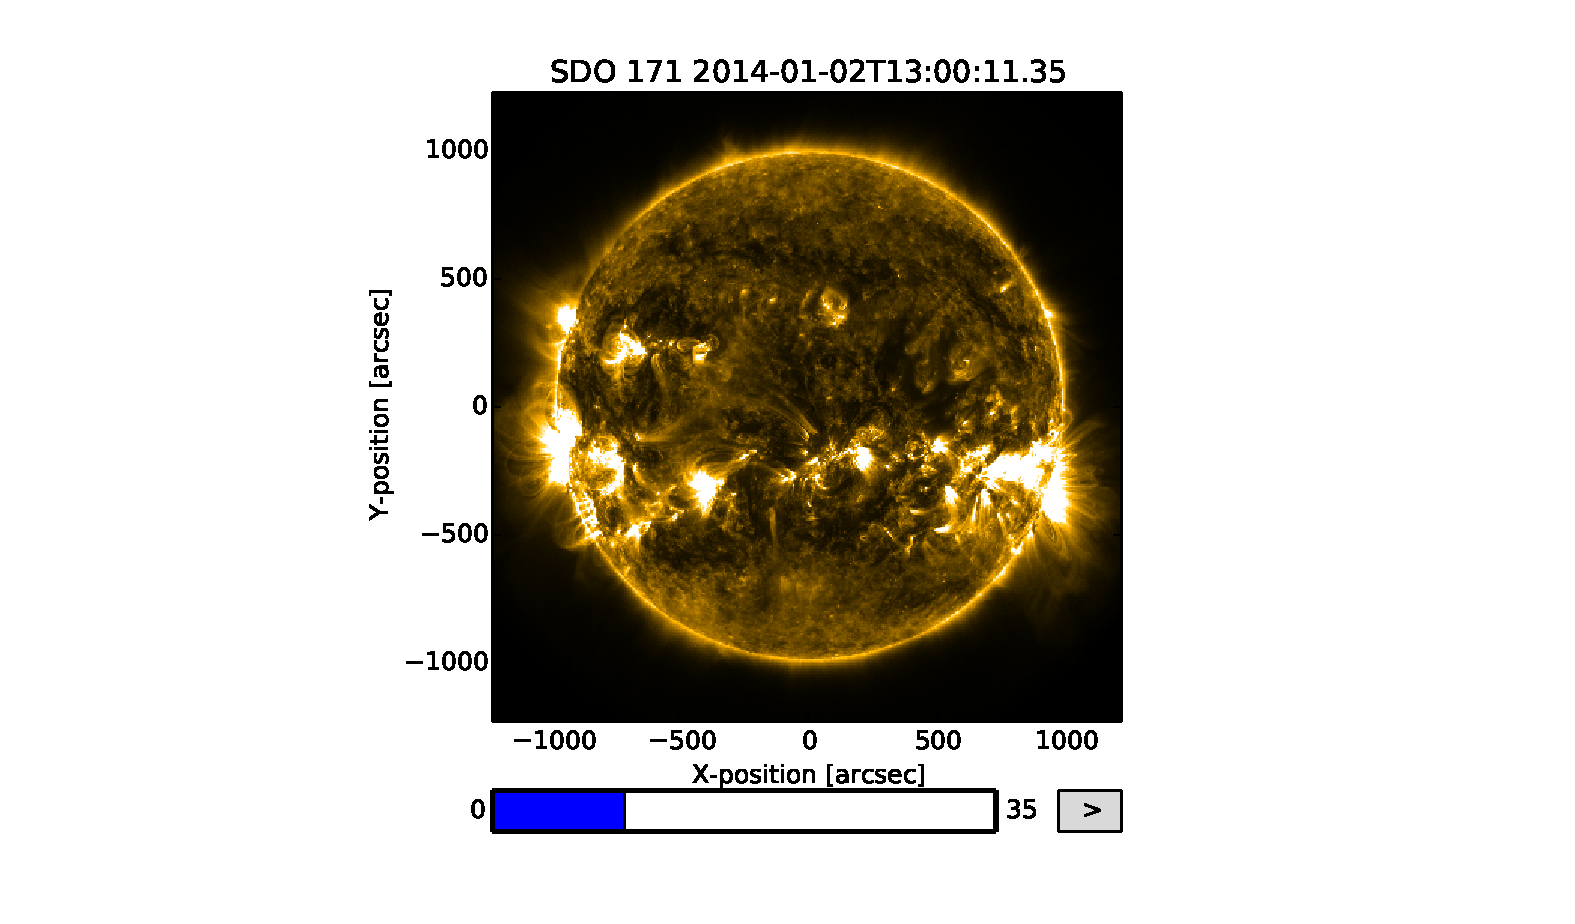
\includegraphics[width=0.8\columnwidth]{aia_cube_controls}
\end{center}
\caption{Example showing the creation of a \texttt{MapCube} from a list of AIA image files. The 
resultant plot makes use of \texttt{matplotlib}'s interactive widgets to allow scrolling 
through the \texttt{MapCube}.}
\label{code:mapcube_1}
\end{listing}
